
Functions of human genes are often studied indirectly, by studying
model organisms such as the mouse \citep{Davis04, Joyce06}. Orthologs
are genes in different species that originate from a single gene in
the last common ancestor of these species. Such genes have often
retained identical biological roles in the present-day organisms, and
are likely to share the function \citep{Fitch70}. Mutations in the
genomic DNA sequence are a key mechanism in evolution. Consequently,
DNA sequence similarity can provide hypotheses of gene function in
poorly annotated species. An exceptional level of conservation may
highlight critical physiological similarities between species, whereas
divergence can indicate significant evolutionary changes
\citep{Jordan05}. Investigating evolutionary conservation and
divergence will potentially lead to a deeper understanding of what
makes each species unique.  Evolutionary changes primarily target the
structure and sequence of genomic DNA. However, not all changes will
lead to phenotypic differences.  On the other hand, sequence
similarity is not a guarantee of functional similarity because small
changes in DNA can potentially have remarkable functional
implications.

Therefore, in addition to investigating {\it structural conservation}
of the genes at the sequence level, another level of investigation is
needed to study {\it functional conservation} of the genes and their
regulation, which is reflected at the transcriptome \citep{Jimenez02,
  Jordan05}. Transcriptional regulation of the genes is a key
regulatory mechanism that can have remarkable phenotypic consequences
in highly modular cell-biological systems \citep{Hartwell99} even when
the original function of the regulated genes would remain intact.

Systematic comparison of transcriptional activity between different
species would provide a straightforward strategy for investigating
conservation of gene regulation \citep{Bergmann04, Enard02, Zhou04}.
However, direct comparison of individual genes between species may not
be optimal for discovering subtle and complex dependency structures.
The associative clustering principle (AC), introduced in
Publications~\ref{ECML}-\ref{AC}, provides a framework for detecting
groups of orthologous genes with exceptional levels of conservation
and divergence in transcriptional activity between two species. While
standard dependency detection methods for continuous data, such as the
generalized singular value decomposition \citep[see e.g.][]{Alter03}
or canonical correlation analysis \citep{Hotelling36} detect global
linear dependencies between observations, AC searches for dependent,
local groupings to reveal gene groups with exceptional levels of
conservation and divergence in transcriptional activity.  The model is
free of particular distributional assumptions about the data, which
helps to allocate modeling resources to detecting dependent subgroups
when variation within each group is less relevant for the analysis.
The remainder of this section provides an overview of the associative
clustering principle and its application to studying evolutionary
divergence between species.

\begin{figure}[t]
\label{fig:acprinciple}
\centerline{
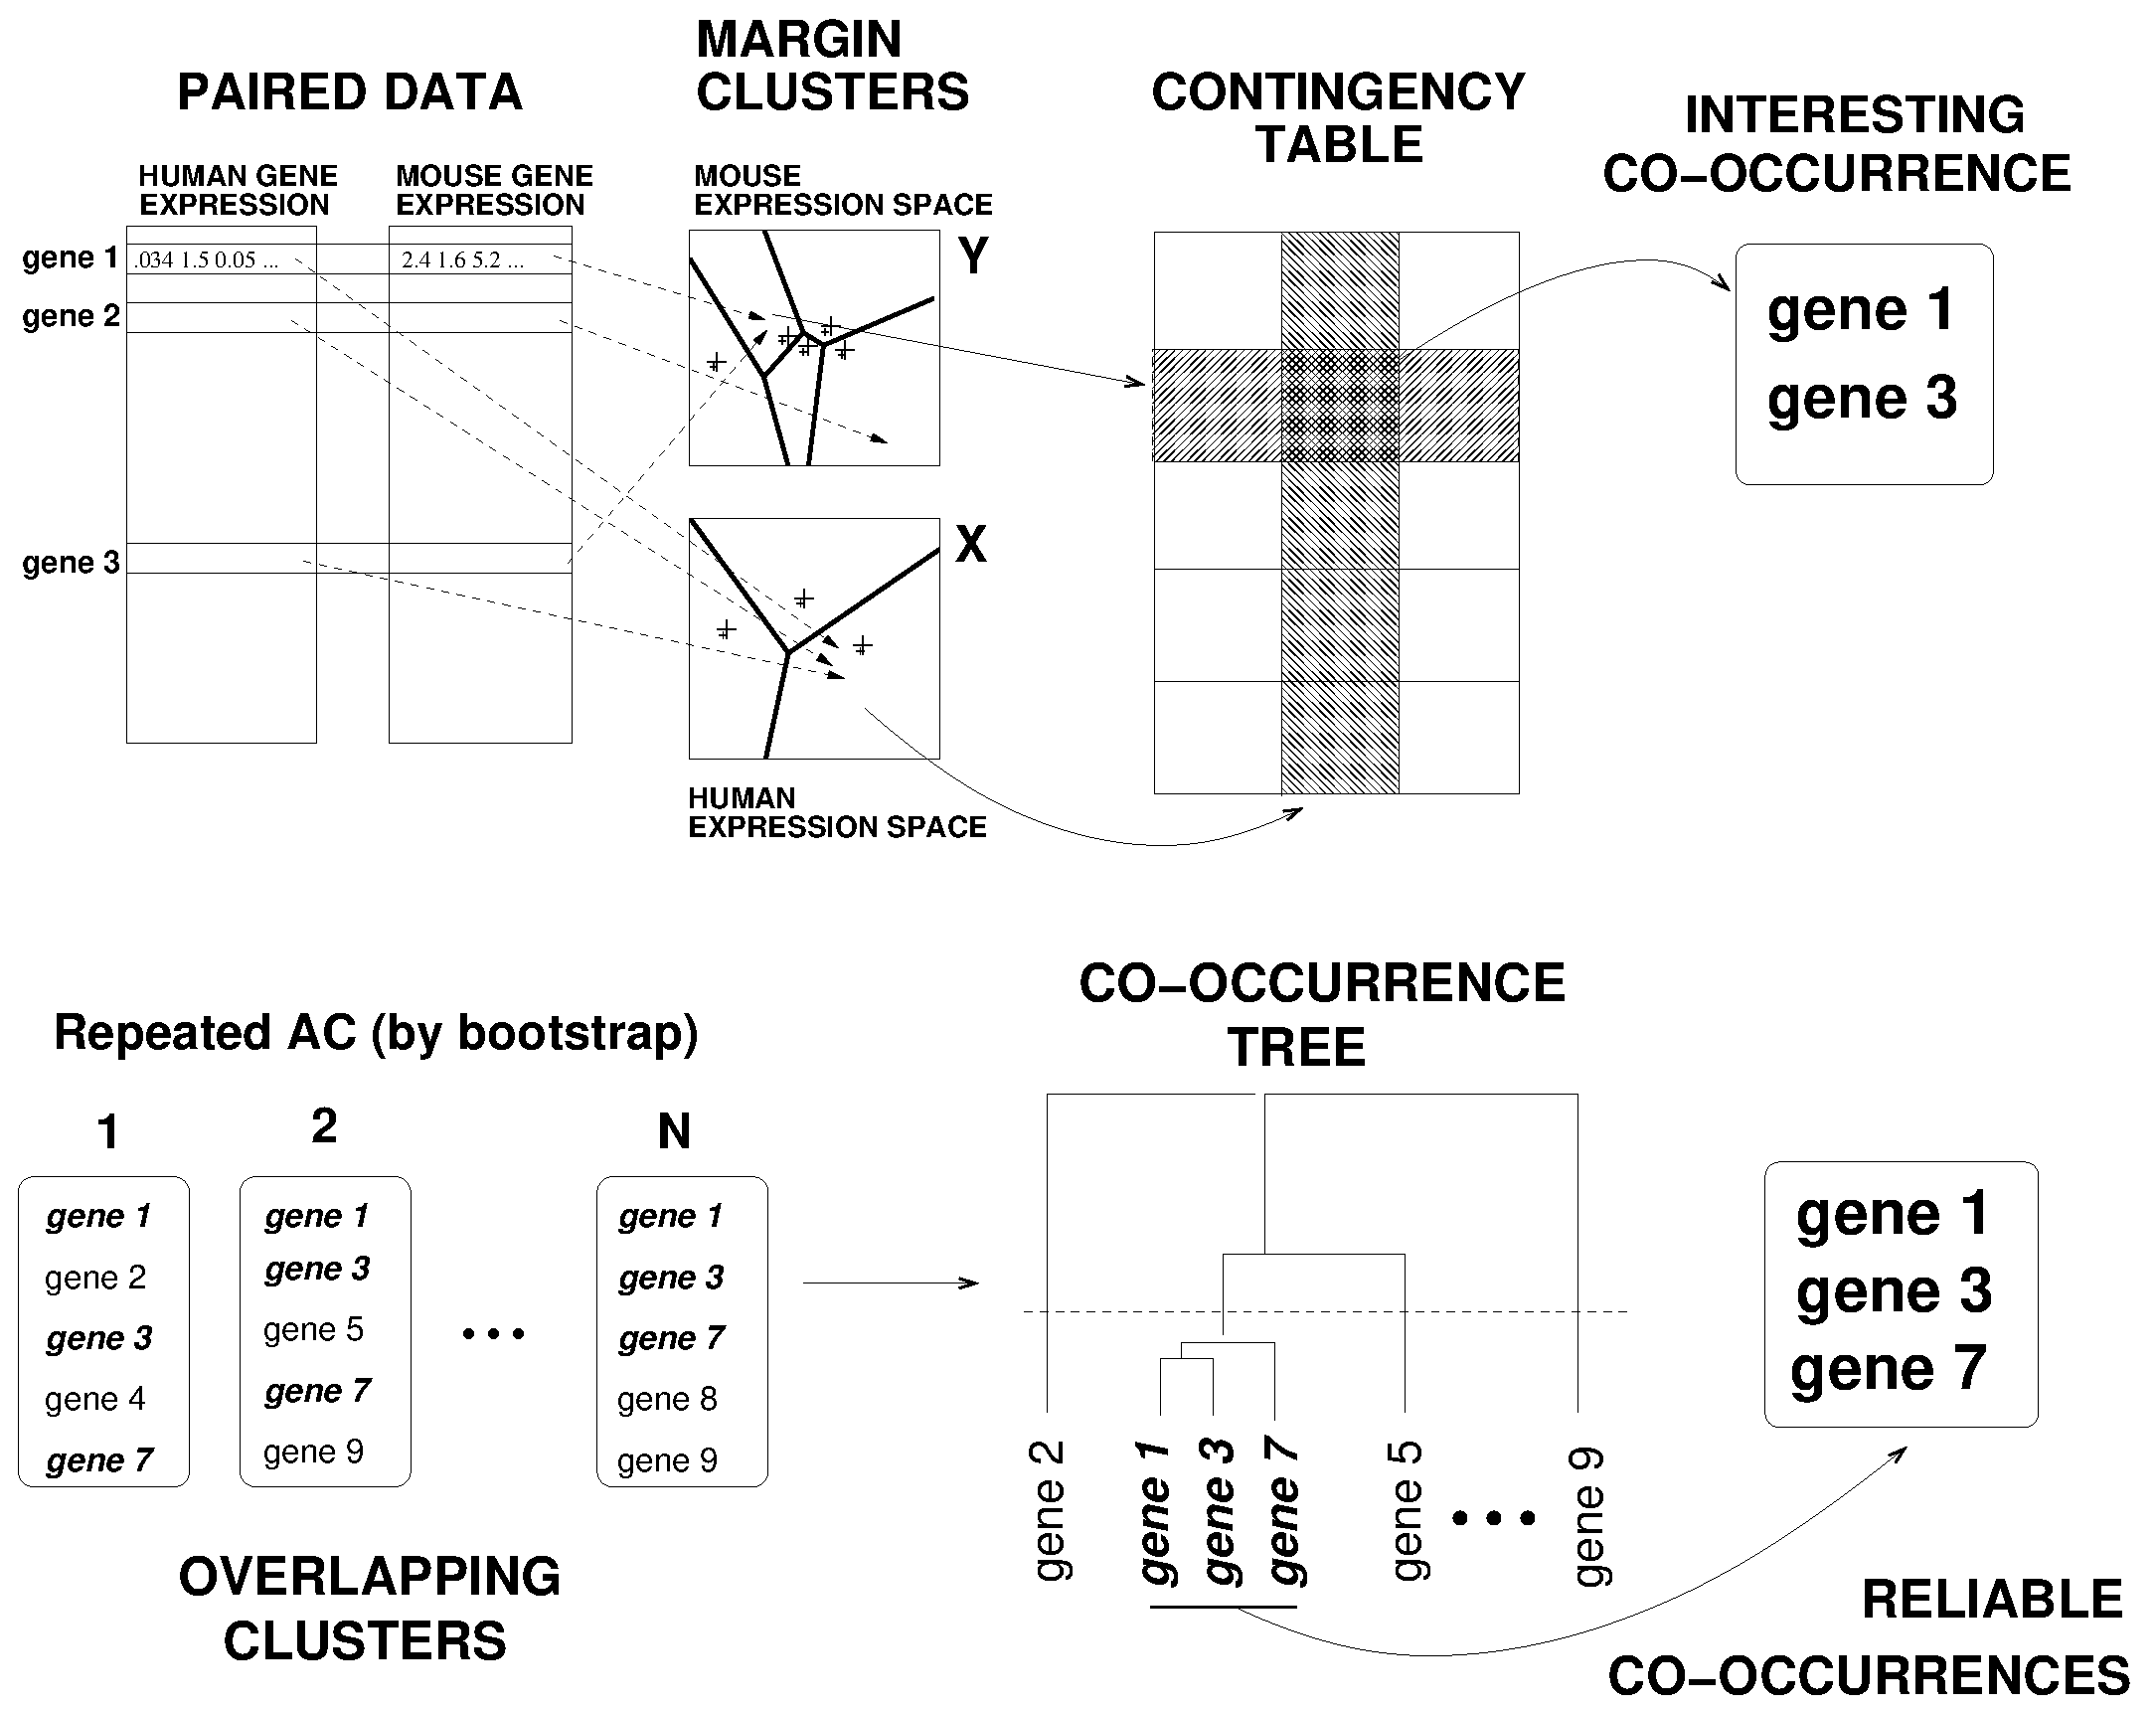
\includegraphics[width=0.9\textwidth]{pic/settingbs.eps}}
\caption{Principle of associative clustering (AC). AC performs
  simultaneous clustering of two data sets, consisting of paired
  observations, and seeks to maximize the dependency between the two
  sets of clusters.  The clusters are defined by cluster centroids in
  each data space.  The clustering results are represented on a
  contingency table, where clusters of the two data sets correspond
  with the rows and columns of the contingency table,
  respectively. These are called the margin clusters of the
  contingency table. The table cells are called cross clusters and
  they contain orthologous genes from the two data sets.  The cluster
  centroids are optimized to produce a contingency table with maximal
  dependency between the margin cluster counts.  Cross clusters that
  show significant deviation from the null hypothesis of independent
  margins indicate dependency. In order to enhance the reliability of
  the results, the clustering is repeated with slightly differing
  bootstrap samples. Then reliable co-occurrences are identified from
  a co-occurrence tree with a specified threshold. Frequently
  co-occurring orthologues are selected for further analyzes.}
\end{figure}

\subsubsection{The associative clustering principle}

The principle of associative clustering (AC) is illustrated in
Figure~\ref{fig:acprinciple}. AC performs simultaneous clustering of
two data sets to reveal maximally dependent cluster structure between
two sets of observations. The clusters are defined in each data space
by {\it Voronoi parameterization}, where the clusters are defined by
cluster centroids to produce connected, internally homogeneous
clusters.  Let us denote the two sets of clusters by
\(\{V^{(x)}_i\}_i\), \(\{V^{(y)}_j\}_j\).  A given data point \(\x\)
is then assigned to the cluster corresponding to the nearest centroid
\(\m_i\) in the feature space, with respect to a given distance
measure\footnote{\(\x \in V_i^{(x)}\) if \(d(\x, \m_i) \leq d(\x,
  \m_k)\) for all \(k\).}  \(d\).  This divides the space into
non-overlapping {\em Voronoi regions}. The regions define a clustering
for all points of the data space. The association between the clusters
of the two data sets can be represented on a contingency table, where
the rows and columns correspond to clusters in the first and second
data set, respectively. The clusters in each data set are called {\it
  margin clusters}. Each pair of co-occurring observations $(\xi,\yi)$
maps to one margin cluster in each data set, and each contingency
table cell corresponds to a pair of margin clusters. These are called
{\it cross clusters}.

AC searches for a maximally dependent cluster structure by optimizing
the Voronoi centroids in the two data spaces in such a way that the
dependency between the contingency table margins is maximized. Let us
denote the number of samples in cross cluster \(i, j\) by
\(n_{ij}\). The corresponding margin cluster counts are $n_{i \cdot} =
\sum_j n_{ij}$ and $n_{\cdot j} = \sum_i n_{ij}$.  The observed sample
frequencies over the contingency table margins and cross-clusters are
assumed to follow multinomial distribution with latent parameters
\(\bth_i, \bth_j\) and \(\bth_{ij}\), respectively.  Assuming the
model $M_I$ of {\it independent margin clusters}, the expected sample
frequency in each cross cluster is given by the outer product of
margin cluster frequencies.  The model $M_d$ of \emph{dependent margin
  clusters} deviates from this assumption. The {\it Bayes factor (BF)}
is used to compare the two hypotheses of dependent and independent
margins. This is a rigorously justified approach for model comparison,
which indicates whether the observations provide superior evidence for
either model. Evidence is calculated over all potential values of the
model parameters, marginalized over the latent frequencies. In a
standard setting, the Bayes factor would be used to compare evidence
between the dependent and independent margin cluster models for a
given clustering solution. AC uses the Bayes factor in a non-standard
manner; as an objective function to maximize by optimizing the cluster
centroids in each data space; the centroids define the margin clusters
and consequently the margin cluster dependencies.

The centroids are optimized with a conjugate-gradient algorithm after
smoothing the cluster borders with continuous parameterization. The
hyperparameters $n^{(d)}$, $n^{(x)}$, and $n^{(y)}$ arise from
Dirichlet priors of the two multinomial models \(M_I\), \(M_D\) of
independent and dependent margins, respectively.  Setting the
hyperparameters to unity yields the classical hypergeometric measure
of contingency table dependency \citep{Fisher34,Yates34}. With large
sample size, the logarithmic Bayes factor approaches mutual
information \citep{Sinkkonen05tr}. The Bayes factor is a desirable
choice especially with a limited sample size since a marginalization
over the latent variables makes it robust against uncertainty in the
parameter values, and because finite contingency table counts would
give a biased estimate of mutual information.  The number of clusters
in each data space is specified in advance, typically based on the
desired level of resolution. Nonparametric extensions, where the
number of margin clusters would be inferred automatically from the
data form one potential topic for further studies; a closely related
approach was recently proposed in \cite{Rogers2010}.

Publication~\ref{AC} introduces an additional, bootstrap-based
procedure to assess the reliability of the findings
(Figure~\ref{fig:acprinciple}). The analysis is repeated with similar,
but not identical training data sets obtained by sampling the original
data with replacement. The most frequently detected dependencies are
then investigated more closely. The analysis will emphasize findings
that are not sensitive to small variations in the observed data.

\subsubsection{Comparison methods}

Associative clustering was compared with two alternative methods:
standard K-means on each of the two data sets, and a combination of
K-means and information bottleneck (K-IB). K-means \citep[see
e.g.][]{Bishop06} is a classical clustering algorithm that provides
homogeneous, connected clusters based on Voronoi
parameterization. Homogeneity is desirable for interpretation, since
the data points within a given cluster can then be conveniently
summarized by the cluster centroid. On the other hand, K-means
considers each data set independently, which is suboptimal for the
dependency modeling task. The two sets of clusters obtained by
K-means, one for each data space, can then be presented on a
contingency table as in associative clustering.  The second comparison
method is K-IB introduced in Publication~\ref{ECML}. K-IB uses K-means
to partition the two co-occurring, continuous-valued data sets into
discrete atomic regions where each data point is assigned in its own
singleton cluster. This gives two sets of atomic clusters that are
mapped on a large contingency table, filled with frequencies of
co-occurring data pairs $(\x_k, \y_k)$. The table is then compressed
to the desired size by aggregating the margin clusters with the
symmetric IB algorithm in order to maximize the dependency between the
contingency table margins \citep{Friedman01}.  Aggregating the atomic
clusters provides a flexible clustering approach, but the resulting
clusters are not necessarily homogeneous and they are therefore
difficult to interpret.

AC compared favorably to the other methods.  While AC outperformed the
standard K-means in dependency modeling, the cluster homogeneity was
not significantly reduced in AC. The cross clusters from K-IB
\citep{Sinkkonen03tr} were more dependent than in AC. On the other
hand, AC produced more easily interpretable localized clusters, as
measured by the sum of intra-cluster variances in
Publication~\ref{AC}. Homogeneity makes it possible to summarize
clusters conveniently, for instance by using the mean expression
profiles of the cluster samples, as in Figure~\ref{fig:ctable}B.
While K-means searches for maximally homogeneous clusters and K-IB
searches for maximally dependent clusters, AC finds a successful
compromise between the goals of dependency and homogeneity.

\begin{figure}[t]
\centerline{
\begin{tabular}{cc}
{\bf A}&{\bf B}\\
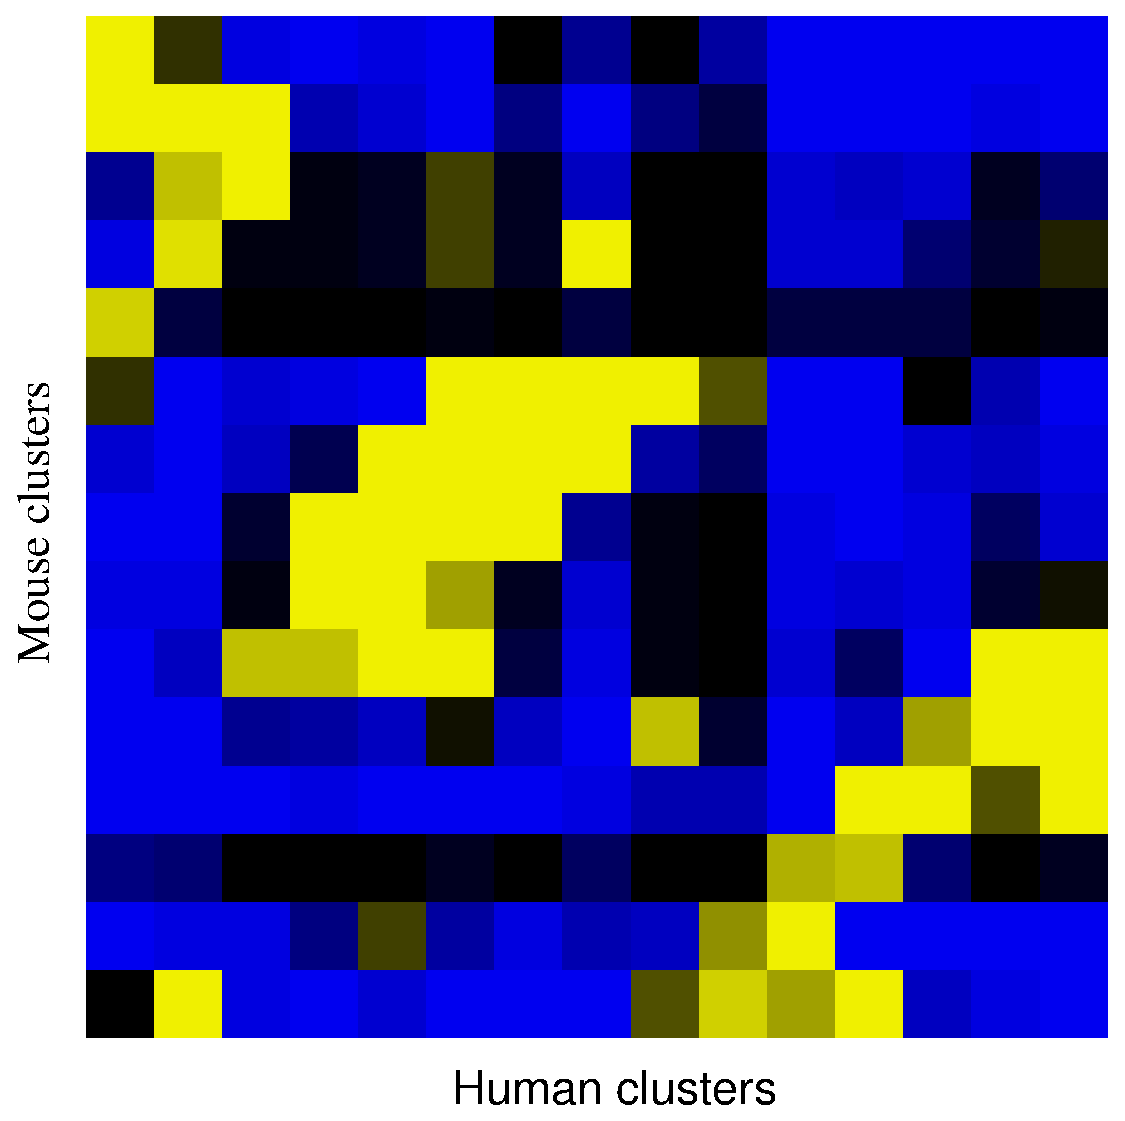
\includegraphics[width=0.4\textwidth]{pic/ctable.eps}& 
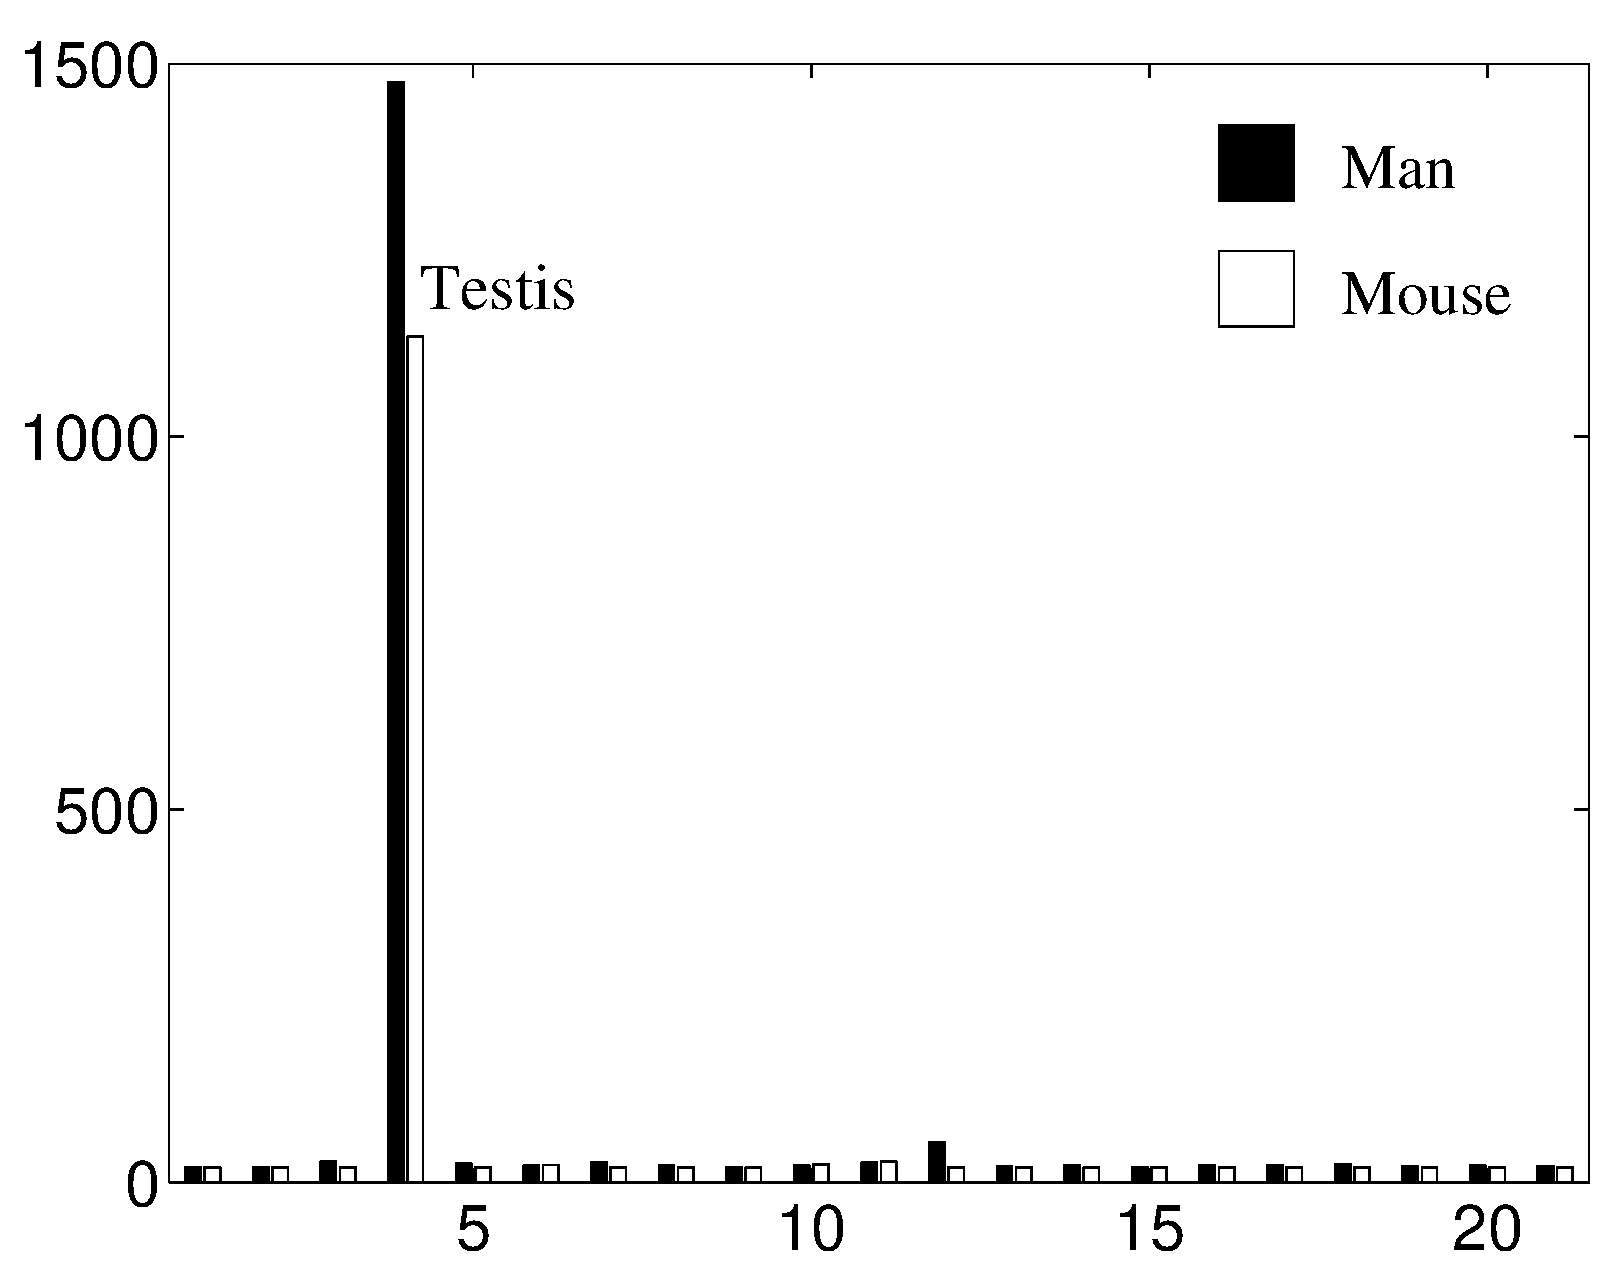
\includegraphics[width=0.5\textwidth]{pic/testis.eps}
\end{tabular}
}
\caption{{\bf A} The contingency table of associative clustering
  highlights orthologous gene groups in human (rows) and mouse
  (columns) with exceptional levels of conservation (yellow) or
  divergence (blue) in transcriptional activity between the two
  species. {\bf B} Average expression profiles of a highly conserved
  group of testis-specific genes across 21 tissues in man and
  mouse. \copyright IEEE. Reprinted with permission from
  Publication~\ref{AC}.}
\label{fig:ctable}
\end{figure}
%/share/mi/mi/papers/bioinf_conf04/manmouse/pic



\subsection{Exploratory analysis of transcriptional divergence between
  species}

Associative clustering is used in Publications~\ref{ECML} and~\ref{AC}
to investigate conservation and divergence of transcriptional activity
of 2818 orthologous human-mouse gene pairs across an organism-wide
collection of transcriptional profiling data covering 46 and 45 tissue
types in human and mouse, respectively \citep{Su02}. AC takes as input
two gene expression matrices with orthologous genes, one for each
species, and returns a dependency-maximizing clustering for the
orthologous gene pairs.  Interpretation of the results focuses on
unexpectedly large or small cross clusters revealed by the contingency
table analysis of associative clustering. Compared to plain
correlation-based comparisons between the gene expression profiles, AC
can reveal additional cluster structure, where genes with similar
expression profiles are clustered together, and associations between
the two species are investigated at the level of such detected gene
groups. The dependency between each pair of margin clusters can be
characterized by comparing the respective margin cluster centroids
that provide a compact summary of the samples within each cluster.

Biological interpretation of the findings, based on enrichment of Gene
Ontology (GO) categories \citep{Ashburner00}, revealed genes with
strongly conserved and potentially diverged transcriptional
activity. The most highly enriched categories were associated with
ribosomal functions, the high conservation of which has also been
suggested in earlier studies \citep{Jimenez02}; ribosomal genes often
require coordinated effort of a large group of genes, and they
function in cell maintenance tasks that are critical for species
survival.  An exceptional level of conservation was also observed in a
group of testis-specific genes, yielding novel functional hypotheses
for certain poorly annotated genes within the same cross-cluster
(Figure~\ref{fig:ctable}). Transcriptional divergence, on the other
hand, was detected for instance in genes related to embryonic
development.

While general-purpose dependency exploration tools may not be optimal
for studying the specific issue of transcriptional conservation, such
tools can reveal dependency with minimal prior knowledge about the
data. This is useful in functional genomics experiments where little
prior knowledge is available. In Publications~\ref{ECML} and~\ref{AC},
associative clustering has been additionally applied in investigating
dependencies between transcriptional activity and transcription factor
binding, another key regulatory mechanism of the genes.
